\documentclass[11pt]{article}
\usepackage[utf8]{inputenc}

% MATH
\usepackage{amssymb}
\usepackage{amsmath}
\usepackage{amsthm}
\usepackage{mathtools}

\newtheorem{pb}{Problème}
\newtheorem{rmq}{Remarque}
%\newtheorem{cusdef}{Def}
%\newtheorem{custhm}{Thm}
%\newtheorem{cuscor}{Cor}
%\newtheorem{cusrk}{Rk}
\newenvironment{cusenv}[2]
{\begin{samepage}\noindent\textbf{#1} -- (#2) \par}
{\end{samepage} \bigskip}

\newenvironment{cusdef}[1]
{\begin{cusenv}{Def}{#1}}{\end{cusenv}}

\newenvironment{custhm}[1]
{\begin{cusenv}{Thm}{#1}}{\end{cusenv}}

\newenvironment{cuscor}[1]
{\begin{cusenv}{Cor}{#1}}{\end{cusenv}}

\newenvironment{cusprop}[1]
{\begin{cusenv}{Prop}{#1}}{\end{cusenv}}

\newenvironment{cusrk}[1]
{\begin{cusenv}{Rk}{#1}}{\end{cusenv}}	

% MISE EN FORME
\usepackage[left=2cm,right=2cm,top=2cm,bottom=2cm]{geometry}

\usepackage{hyperref}
\usepackage{xcolor}
\hypersetup{
	colorlinks,
	linkcolor={red!50!black},
	citecolor={blue!50!black},
	urlcolor={blue!80!black}
}


% MACROS
\usepackage{xparse}
\newcommand{\smbox}[1]{\mbox{\footnotesize #1}}
\newcommand{\A}{\mathcal{A}}
\newcommand{\Am}{\mathbb{A}}
\newcommand{\N}{\mathbb{N}}
\newcommand{\C}{\mathbb{C}}
\renewcommand{\P}{\mathbb{P}}
\newcommand{\R}{\mathbb{R}}
\newcommand{\K}{\mathbb{K}}
\newcommand{\M}{\mathbb{M}}
\newcommand{\Ah}{A^{hom}}
\newcommand{\uh}{u^{hom}}
\newcommand{\fh}{f^{hom}}


\newcommand{\ie}{\emph{i.e.} }
\newcommand{\ms}{~~~}
\newcommand{\norm}[1]{\left|\left|#1\right|\right|}
\newcommand{\dual}[1]{#1'}
\newcommand{\sca}[2]{\big<#1, #2\big>}
\newcommand{\cont}[1]{\mathcal{C}^{#1}}
\newcommand{\question}[2]{\paragraph{Question #1.}\textit{#2} \\}
\newcommand{\Hd}{H^1_{\#}}



\title{Rapport TP X01 \\ TP3}
\author{Aurélien Valade}
\date{}

\begin{document}
\maketitle

\section{Introduction et structure du code}


Le but de ce TP est de résoudre le problème suivant :

\begin{pb}[$\varepsilon-$problème]
  \label{pb:eps}
  Soit $\varepsilon>0$, soient $A^\varepsilon, ~f^\varepsilon$ bien définies, trouver $u^\varepsilon\in H^1_0(\Omega)$ tel que  
  \[
    \begin{cases}
      \nabla \big(A^\varepsilon(x,x/\varepsilon) \nabla u^\varepsilon\big) = f^\varepsilon(x, x/\varepsilon) \quad \mbox{sur}\quad \Omega\\
      u^\varepsilon = 0 \quad \mbox{sur}\quad \partial\Omega.
    \end{cases}
  \]
\end{pb}
\begin{rmq}
  On a $x =(x_1, x_1) \in \R^2$ et $x/\varepsilon \equiv y = (y_1, y_2) \in [0,1]^2$ car les fonctions sont périodiques par rapport à leur seconde
  variable. Dans la suite on note $Y=[0,1]^2$ la cellule élémentaire sur laquelle les coefficients de $A^\varepsilon$ sont périodiques. Dans les cas ou on
  ne travaille que sur une cellule on prend $\varepsilon=1$ et on note $A := A^1$.
\end{rmq}
\begin{pb}
  \label{pb:hom}
  Trouver $u^0 \in H^1_0(\Omega)$ solution du $\varepsilon-$problème \ref{pb:eps} à la limite $\varepsilon\to 0 $.
  \[
    \begin{cases}
      \nabla \big(\Ah(x) \nabla \uh\big) = \fh(x) \quad \mbox{sur}\quad \Omega\\
      \uh= 0 \quad \mbox{sur}\quad \partial\Omega.
    \end{cases}
  \]
\end{pb}


Pour cela nous allons d'abord calculer numériquement les solutions du problème \ref{pb:eps} pour plusieurs valeurs de $\varepsilon>0$. Dans un second temps nous
introduirons les problèmes de cellules que nous résoudrons numériquement, puis nous pourrons enfin calculer la solution au problème \ref{pb:hom}.

La structure du code ainsi que l'arrangement des dossiers ont été un peu modifiés. Tous les \texttt{*.msh} pour les problèmes de Neumann ou Dirichlet
se trouvent dans le dossier \texttt{geoms/} avec un executable \texttt{bash} pour en créer à volonté. Les \texttt{*.msh} pour les problèmes
périodiques se trouvent eux dans le dossier \texttt{geoms\_per/} de même qu'un script pour les générer. On trouve la première partie du TP dans le
dossier \texttt{SolutionExacte/} et la second partie dans le dossier \texttt{SolutionPbHomogeneise/}. 

De plus, le corps de la routine principale se trouve maintenant dans \texttt{principal\_dirichlet\_aux.m}, cependant le fichier script est toujours bien
\texttt{principal\_dirichlet.m}.

\section{Solution exacte}

\subsection{Discrétisation}

Le but de cette partie est d'étudier la convergence effective des solutions numériques vers des solutions analytiques connues. Les résultats présentés ici sont
calculés à partir des routines implémentées pour les TP précédents.

Nous allons donc résoudre le problème \ref{pb:eps} en faisant varier $A^\varepsilon$ et $f^\varepsilon$ de paire de sorte à ce que la solution $u$ soit connue et
ne dépende pas de $\varepsilon$. L'ensemble des matrices de diffusion et leur seconds membres associés se trouvent en \autoref{tab:Af}. Dans tous ces cas on
calcul $f^\varepsilon$ de sorte à ce que la solution soit
\[
  u^\varepsilon(x, y) = u(x, y) = \sin(\pi x)\sin(\pi y).
\]

\begin{table}
  \centering
  \begin{tabular}{c|c|p{0.5\textwidth}}
    type & $A^\varepsilon$ & $f^\varepsilon$ \\
    \hline
    (i) & Id & $2\pi^2\sin(\pi y_1 )\sin(\pi y_2)$ \\
    \hline
    (ii) & $ \left(
           \begin{matrix}
             1 & 0 \\
             0 & 2 
           \end{matrix} \right) $   
                           & $3\pi^2\sin(\pi y_1 )\sin(\pi y_2)$ \\
    \hline
    (iii) & $ \left(
            \begin{matrix}
              2+\sin(2\pi y_1) & 0 \\
              0 & 4 
            \end{matrix} \right)$   
                           & {\small $2\pi^2 (-2 \cos(\pi y_1) \cos(2\pi y_1) +
                             \sin(\pi y_1)\sin(2 \pi y_1) + 3 \sin(\pi y_1))\sin(\pi y_2)$} \\
    \hline
    (iv) & $ \left(
           \begin{matrix}
             2+\sin(2\pi y_1) & 0 \\
             0 & 4+\sin(2\pi y_1)
           \end{matrix} \right)$   
                           & {\small $\pi^2 (-4 \cos(\pi y_1) \cos(2 \pi y_1) + 
                             3 \sin(\pi y_1) \sin(2 \pi y_1) + 6 \sin(\pi y_1)) \sin(\pi y_2)$} \\
    \hline
    (v) & $ ( 2+\sin(2\pi y_1)) ( 4+\sin(2\pi y_2) )$ Id   
                           & {\footnotesize $4 \pi^2                                                                     
                             (- (\sin(2 \pi  y_1) + 1)  \sin(\pi y_1)  \cos(\pi y_2)  \cos(2 \pi  y_2) -
                               (\sin(2 \pi  y_2) + 4)  \sin(\pi y_2)  \cos(\pi y_1)  \cos(2 \pi  y_1) +
                             (\sin(2 \pi  y_1) + 1)  (\sin(2 \pi  y_2) + 4)  \sin(\pi y_1)  \sin(\pi y_2))$} \\
  \end{tabular}
  \caption{Matrices de diffusion et seconds membres associés. Dans un soucie de lisibilité les fonctions sont données pour $\varepsilon=1$. }
  \label{tab:Af}
\end{table}

\subsection{Résultats}

On observe tout d'abord que le code est quasi-exacte dès que la maillage est raisonnablement précis pour les cas (i) et (ii) où les matrices sont
constantes, l'erreur $L^2$ et $H^1$ étant d'environ $10^{-30}$.
Dans les cas ou $A^\varepsilon$ est périodique et $\varepsilon$ est assez grand pour que l'erreur soit bien résolue (cf. paragraphe suivant) l'erreur est bien plus grande mais décroît avec le maillage comme attendu c'est à dire
\begin{itemize}
\item en $1/h^2$ pour l'erreur $L^2$
\item en $1/h$ pour l'erreur $H^1$
\end{itemize}
comme on peut le voir en \autoref{fig:err_msh}. En bleu on voit une courbe pour un $\varepsilon$ où l'erreur est résolue alors qu'en rouge, pour un $\varepsilon$ très
faible, les courbes sont moins monotones. 

\begin{figure}
  \centering
  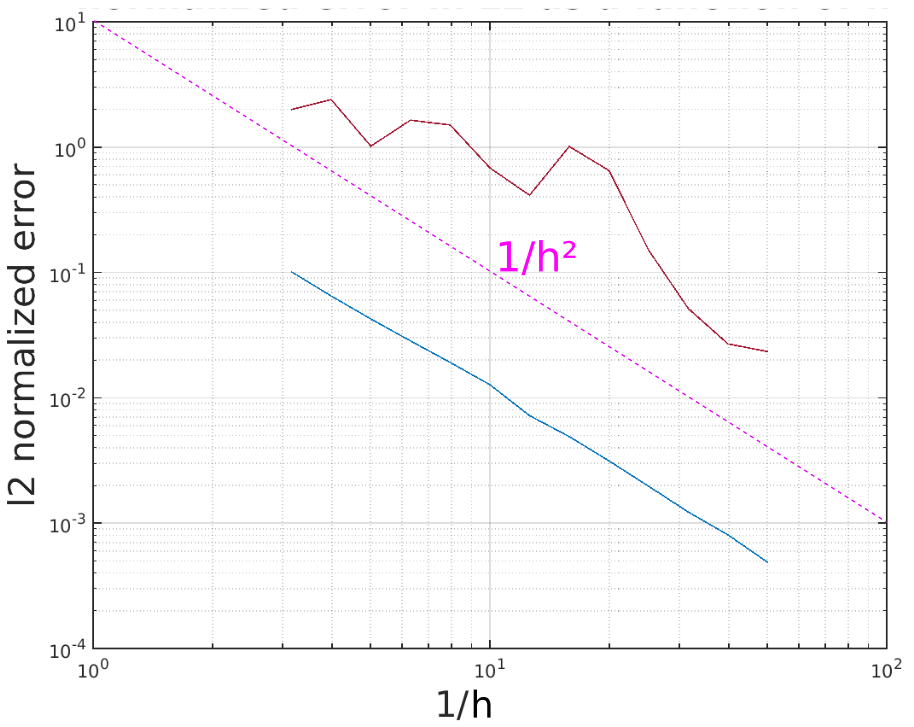
\includegraphics[height=.25\textheight]{SolutionExacte/err_L2} 
  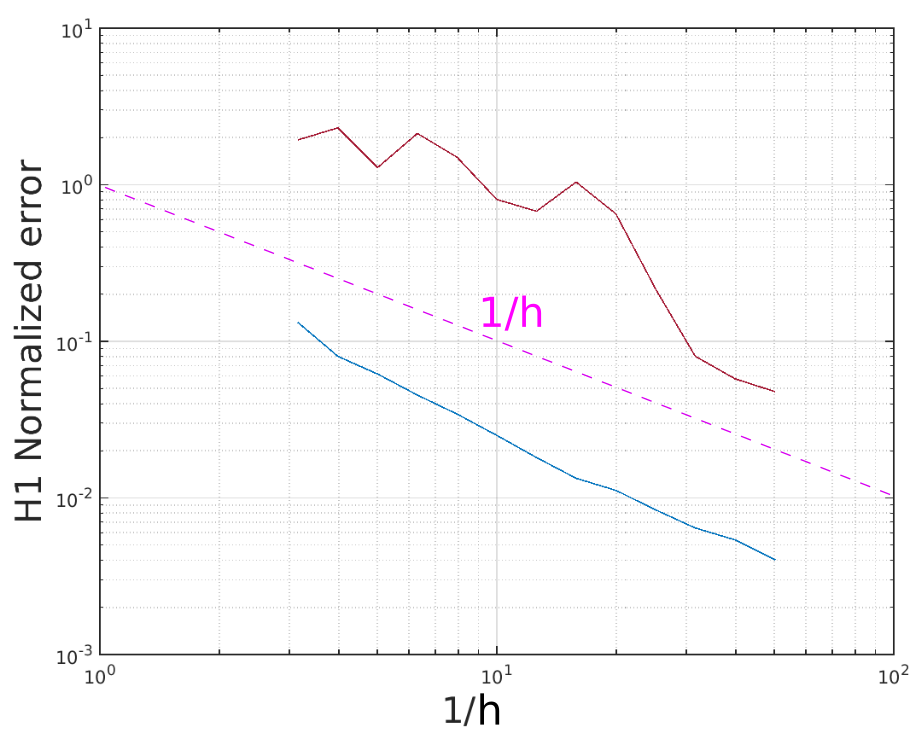
\includegraphics[height=.25\textheight]{SolutionExacte/err_H1} 
  \caption{Erreurs $L^2$ et $H^1$ en fonction du pas du maillage pour $\varepsilon=1$ en bleu et  $\varepsilon=20$ en rouge. On est ici dans le cas
    (iii), mais des courbes similaires sont obtenues dans les cas (iv) et (v). }
  \label{fig:err_msh}
\end{figure}

On peut aussi observer un phénomène intéressant de résolution de l'erreur en fonction du maillage et de $\varepsilon$. Quand $\varepsilon$ tend vers
zéro, la période des oscillation passe sous la taille caractéristique des cellules $h$, et les oscillations attendues disparaissent comme le montre la
\autoref{fig:osc_eps}. Cela amène à des différences qualitatives entre solution numérique et solution exacte \ie le profile de la solution numérique
ne peut plus suivre le profile exact. Il est cependant difficile de repérer ce ``décrochage'' sur les courbes des erreurs $L^2$ et $H^1$ augmentent
très rapidement en fonction de $1/\varepsilon$, puis que plus que linéairement dans un graphe log-log comme on peut le voir en
\autoref{fig:err_eps}.   
\begin{figure}
  \centering
  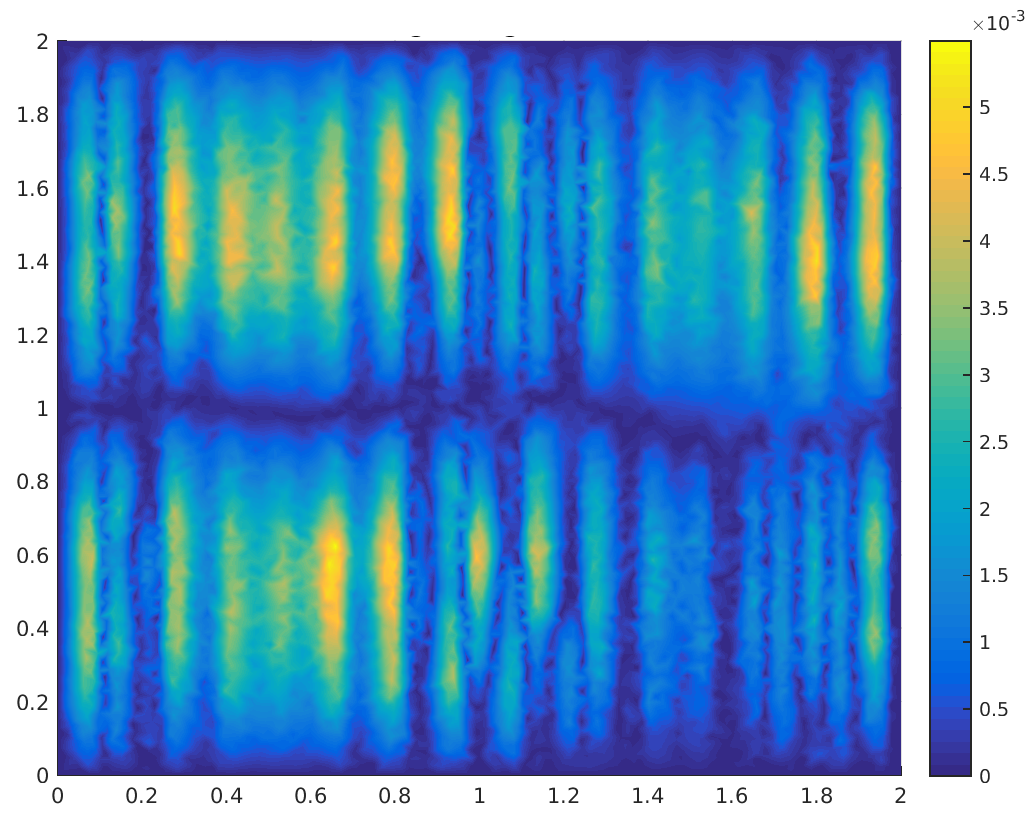
\includegraphics[height=.25\textheight]{SolutionExacte/limit_res_eps7} 
  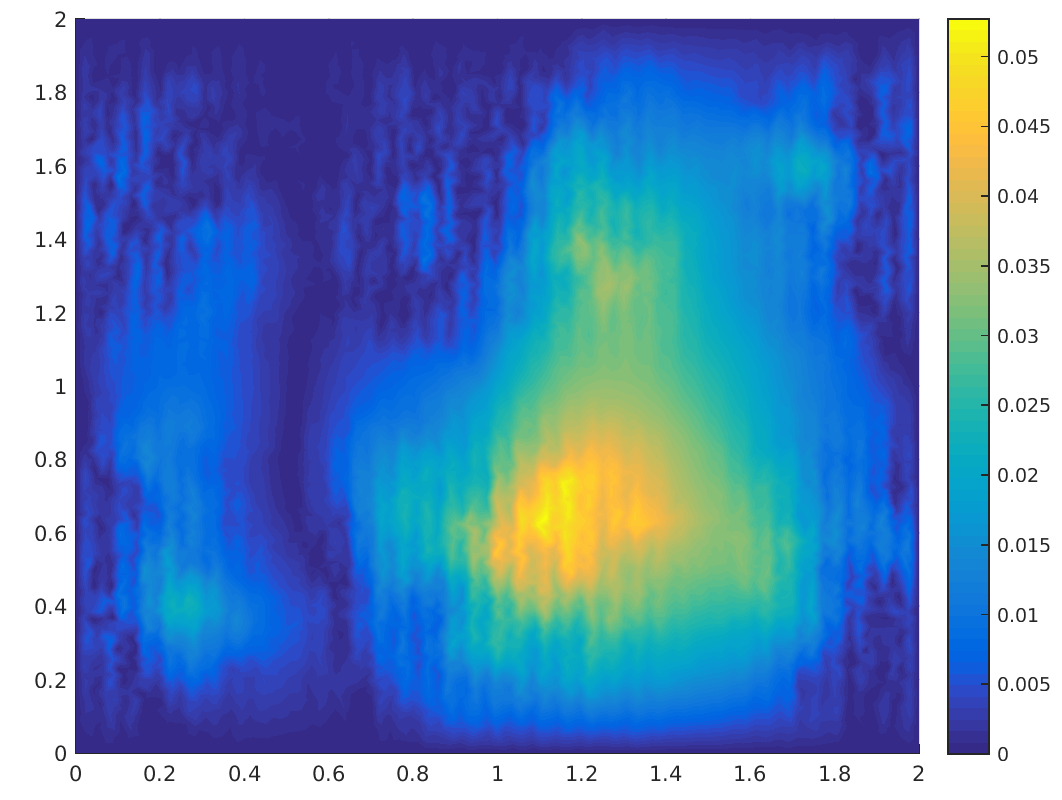
\includegraphics[height=.25\textheight]{SolutionExacte/non_res_eps18}   
  \caption{Différence entre solution numérique et exacte pour $\varepsilon=1/7$ et $\varepsilon=1/18$. Dans le premier cas on voit que les
    oscillations sont approximativement résolues, alors que dans le second cas on ne voit finalement que la moyenne de l'erreur sur plusieurs
    périodes. On a pour ces figures $h=2.5\cdot10^{-2}$ et on est dans le cas (iii).}
  \label{fig:osc_eps}
\end{figure}

\begin{figure}
  \centering
  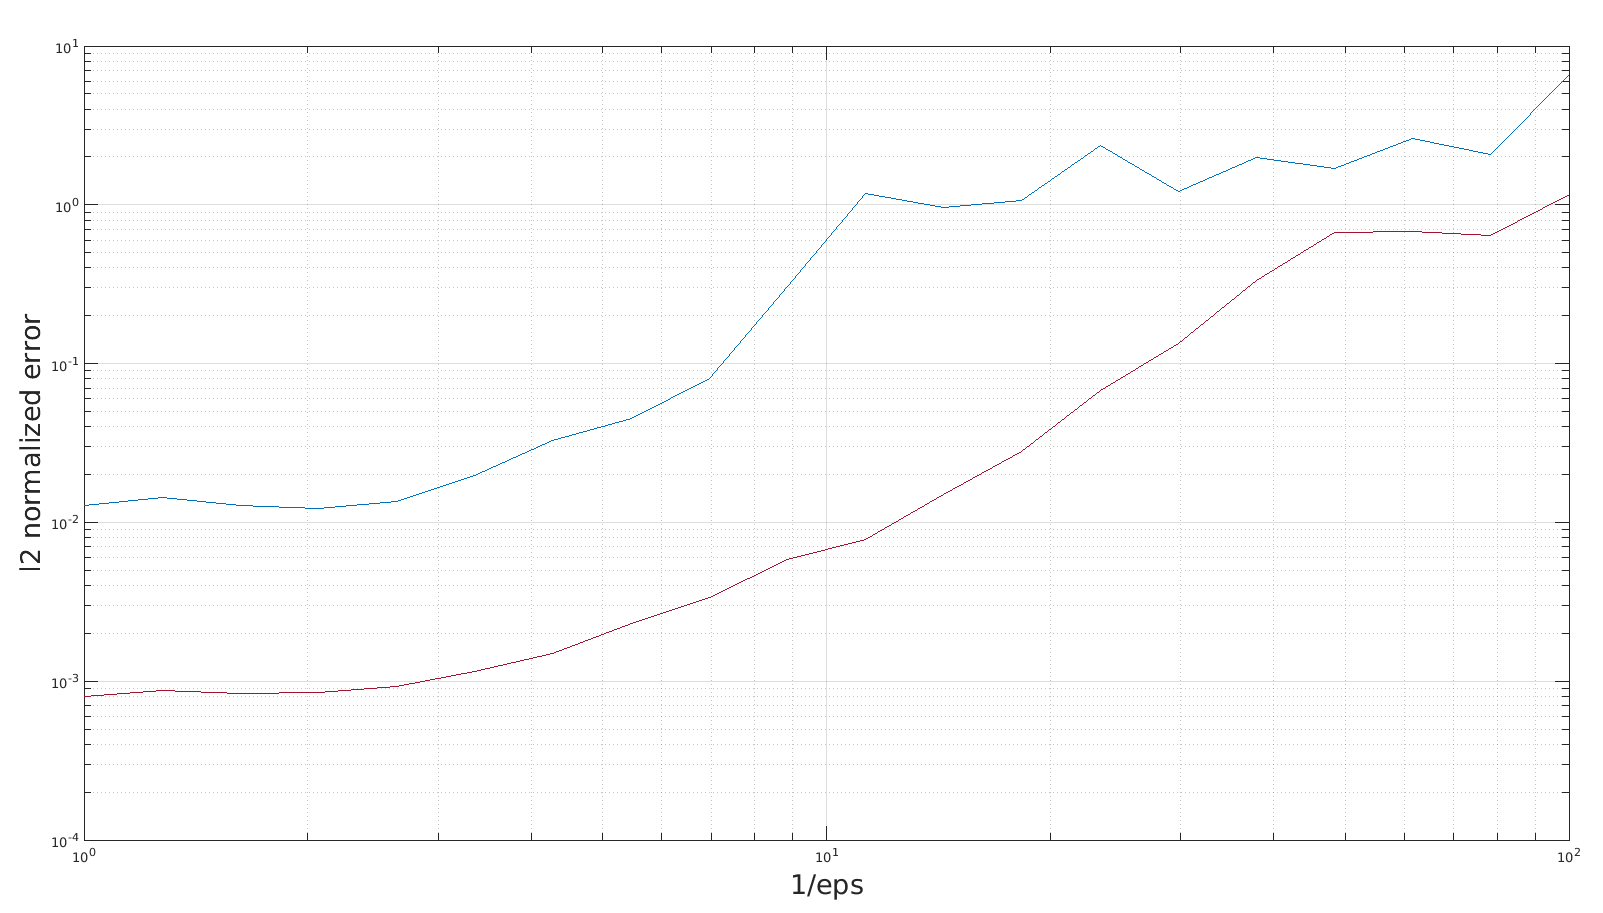
\includegraphics[height=.25\textheight]{SolutionExacte/err_L2_eps} 
  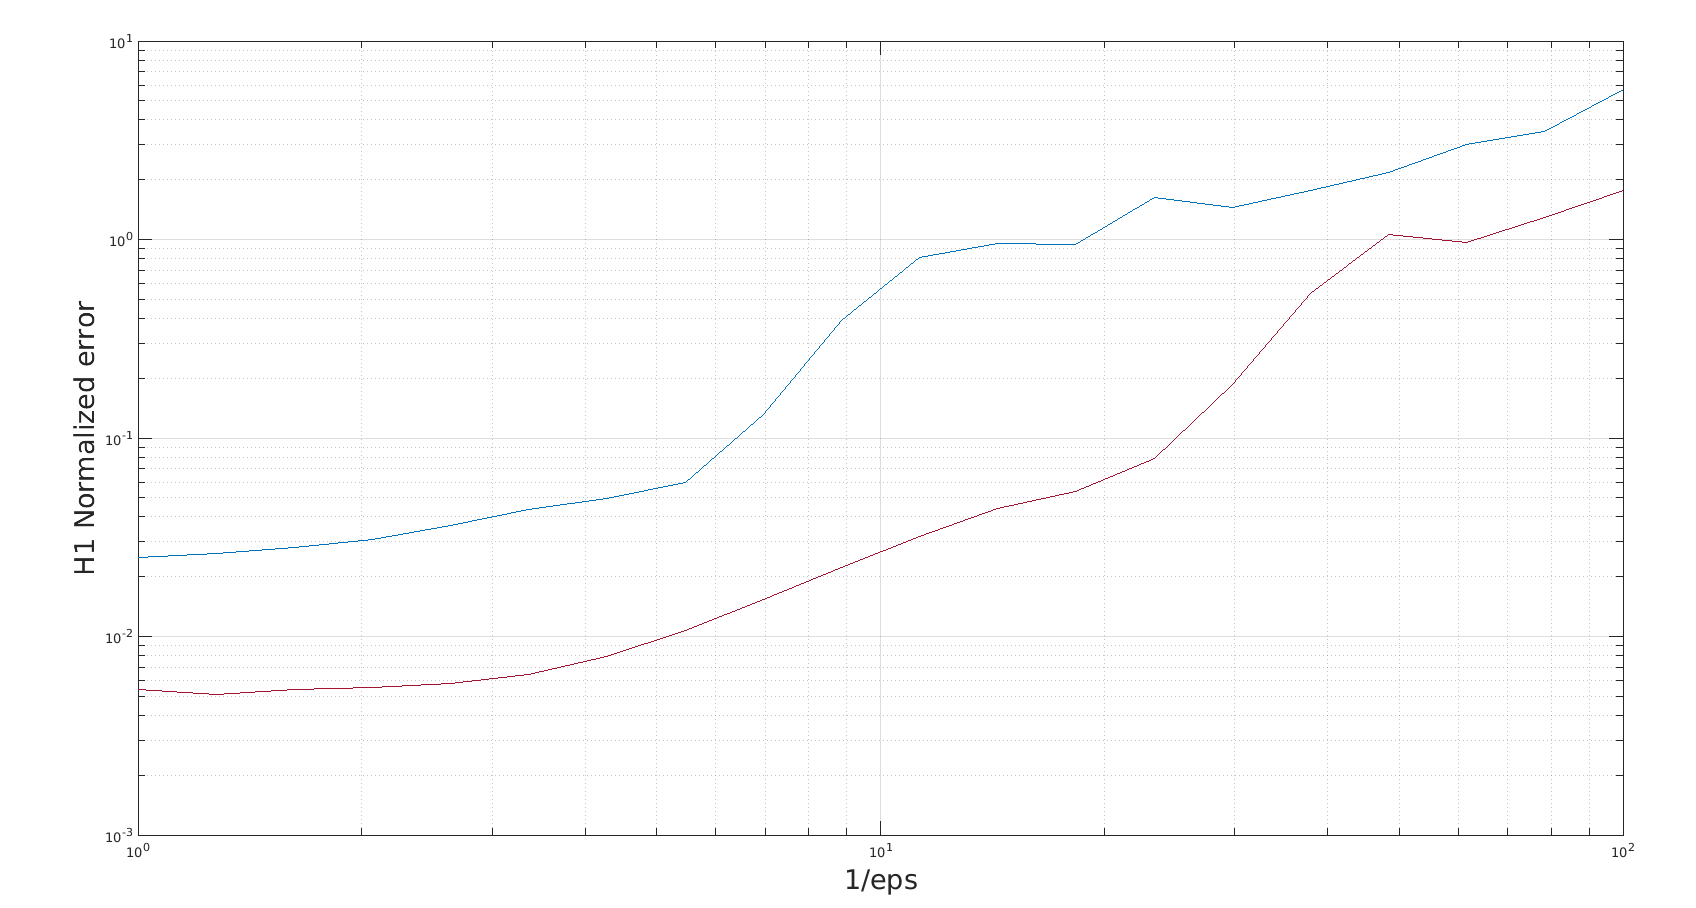
\includegraphics[height=.25\textheight]{SolutionExacte/err_H1_eps}   
  \caption{Erreurs $L^2$ (en haut) et $H^1$ (en bas) en fonction de la taille d'une cellule $\varepsilon$. On trace en bleu pour un maillage avec
    $h=0.1$ et en rouge pour un second maillage avec $h=0.02$. On est ici dans le cas (iii). Il est intéressant de noter que l'erreur relative
    diverge, et atteint sur ce graphe un facteur $10$.}
  \label{fig:osc_eps}
\end{figure}
\section{Solution au problème homogénéisé}

\subsection{Les problèmes de cellule}

La difficulté mathématique à laquelle répond la méthode de l'homogénéisation est le passage du problème \ref{pb:eps} au problème dit homogénéisé
\ref{pb:hom}. Il faut notamment calculer les coefficients limites de $\Ah$ et $\fh$. Pour ce qui concerne $\fh$, comme nous travaillons avec
$A^\varepsilon$ parfaitement périodique, on sait que l'on va avoir $\Ah$ constant, et donc pour garder la solution
\[
  \uh(x, y) = u(x, y) = \sin(\pi x)\sin(\pi y)
\]
il nous suffira de prendre
\[
  \fh = \pi^2 Tir(\Ah) u(x, y).
\]

La difficulté est donc de calculer $\Ah$ à partir de $A$. La théorie de l'homogénéisation nous dit que
\begin{equation}
  \label{eq:Ah}
  \Ah_{ij} = \int_Y \big(A(e_j+\nabla w_j), e_i+\nabla w_i\big)
\end{equation}
ou les $\{w_i\}_{1,2}$ sont les solutions aux problèmes de cellules référés dans le problème \ref{pb:cell} sous leurs
formes variationnelles.
\begin{pb}
  \label{pb:cell}
  Trouver $w_i \in V$ tels que $\forall i \in \{1,2\}$
  \begin{equation}
    \forall \phi \in V, \quad \int_Y A \nabla w_i \nabla v = - \int_Y A e_i \nabla \phi 
  \end{equation}
  avec
  \[
    V = 
    \left\{
      \psi \in \Hd(Y), \qquad \int_Y \psi = 0
    \right\}.
  \]
\end{pb}

Montrons tout d'abord que ces problèmes sont bien posés. On prend l'une des deux équations, et l'on pose $w:=w_i$, de même on pose
\[
  a(w,\phi) = \int_Y A \nabla w \nabla \phi, \quad
  l(\phi) = -\int_Y A e_i \nabla \phi 
\]

On a bien $a(w, \phi)$ et $l(\phi)$ (bi)linéaires. Montrons que $a(w, \phi)$ continue 
\begin{align*}
  \big|a(w,\phi)\big| &= \left| \int_Y A \nabla w \nabla \phi \right| \\
                   &\leq \norm{A\nabla w}_{L^2} \norm{\nabla \phi}_{L^2} && \mbox{Cauchy Schwarz} \\
                   &\leq \beta \norm{\nabla w}_{L^2} \norm{\nabla \phi}_{L^2} && \mbox{A bornée} \\
                   &\leq \beta \norm{w}_{H^1} \norm{\phi}_{H^1} && \norm{\cdot}_{L^2}<\norm{\cdot}_{H^1} \\
\end{align*}

Montrons que $l(\phi)$ est continue
\begin{align*}
  \big|l(\phi)\big| &= \left| \int_Y A e_i \nabla \phi \right|  && \text{définition} \\
                 &\leq \norm{Ae_i}_{L^2} \norm{\nabla \phi}_{L^2} && \text{Cauchy Schwarz} \\
                 &\leq \beta_i \norm{\nabla \phi}_{L^2} && \text{$A$ bornée, donc $A e_i$ aussi} \\
                 &\leq \eta_i \norm{\phi}_{H^1} && \norm{\cdot}_{L^2}<\norm{\cdot}_{H^1}
\end{align*}

Montrons que $a(w, \phi)$ est coercive
\begin{align*}
  a(w,w) &= \int_Y A \nabla w  \nabla w \\
         &\geq \xi \int_Y \nabla w^2  && \text{$A$ minorée par $\xi$}\\
         &\geq \xi \norm{\nabla w}^2_{L^2} \\
         &\geq \zeta \norm{w}^2_{H^1} && \text{Poincaré dans $V$} 
\end{align*}
avec $\zeta = \frac{\xi}{(C^2+1)}$, $C$ étant la constante de Poincaré associée à $V$.

\subsection{Problèmes dégradés}

Cependant, les problèmes étant mal conditionnés sous ces formes, on va plutôt résoudre des problèmes dit dégradés, présentés dans le problème
\ref{pb:celleta}.

\begin{pb}[Problèmes dégradés]
  \label{pb:celleta}
  Soit $\eta>0$. Trouver $w_i \in \Hd$ tels que $\forall i \in \{1,2\}$
  \begin{equation}
    \forall \phi \in V, \quad \int_Y A \nabla w_i \nabla \phi + \eta \int_Y w_i \phi = - \int_Y A e_i \nabla \phi.
  \end{equation}
\end{pb}

À nouveau, on choisie un $i$ et on pose $w:=w_i$, 
\[
  a(w,\phi) = \int_Y A \nabla w \nabla \phi + \eta \int_Y w \phi, \qquad
  l(\phi) = -\int_Y A e_i \nabla \phi
\]

On note qu'en prenant $\phi=1$, on montre que $w$ est d'intégrale nulle. Donc si $w\in\Hd$ résout le problème  \autoref{pb:celleta} alors $w\in V$, et respecte donc Poincaré.  \\
On remarque aussi que $l(\phi)$ reste la même que précédemment, il n'est donc pas nécessaire de refaire les calculs. 

Montrons que $a$ est toujours continue sous cette forme :
\begin{align*}
  \big|a(w,\phi)\big| &\leq \left| \int_Y A \nabla w \nabla \phi \right| + \eta \left| \int_Y  w \phi \right| && \mbox{ineg. triang} \\
                   &\leq \norm{A\nabla w}_{L^2} \norm{\nabla \phi}_{L^2} + \eta \norm{w}_{L^2} \norm{\phi}_{L^2} && \mbox{Cauchy Schwarz} \\
                   &\leq \beta \norm{\nabla w}_{L^2} \norm{\nabla \phi}_{L^2} + \eta \norm{w}_{L^2} \norm{\phi}_{L^2} && \mbox{A bornée} \\
                   &\leq \beta \norm{w}_{H^1} \norm{\phi}_{H^1} + \eta \norm{w}_{H^1} \norm{\phi}_{H^1} && \norm{\cdot}_{L^2}<\norm{\cdot}_{H^1} \\
                   &\leq (\beta + \eta) \norm{w}_{H^1} \norm{\phi}_{H^1}
\end{align*}

Montrons maintenant que $a$ est toujours coercive
\begin{align*}
  a(w,w) &= \int_Y A \nabla w  \nabla w + \eta \int_Y w^2 \\
         &\geq \xi \norm{\nabla w}^2_{L^2} + \eta \norm{w}^2_{L^2} \\
         &\geq \zeta \norm{w}^2_{H^1} + \eta \norm{ w}^2_{L^2} && \text{Poincaré dans }V\\
    \big(&\geq \zeta  \norm{w}^2_{H^1}\big)
\end{align*} 
avec $\zeta = \frac{\xi}{(C^2+1)}$. Quand $\eta$ tend vers zéro on retrouve le résultat de la question 1. En considérant $V = \text{Vect}\big(\{\omega_I\}_{1,N})$, la matrice éléments finis $\Am^{\eta}$ qu'on écrit donc
\[
  \Am^{\eta} = \K + \eta \M 
\]
avec
\[
  \K \in \R^{N\times N},\quad \K_{IJ} = \int A \nabla \omega_I \nabla \omega_J,  \\
  \M \in \R^{N\times N},\quad \M_{IJ} = \int \omega_I \omega_J
\]
tend vers la matrice $\K$ quand $\eta$ tend vers $0$ avec une vitesse \emph{a priori} proportionelle à $\eta$.

Il nous faut maintenant prouver que le problème dégradé est équivalent au problème de cellule initiale quand $\eta$ tend vers zéro. On va précisément démontrer
que
\[
  \forall i \in \{1,2\}, \exists C>0 ~tq~ \norm{w_i-w_i^\eta}_{H^1} < C \eta.
\]
En sommant les équations des problèmes \autoref{pb:cell} et \autoref{pb:celleta}, on a
\[
  \int_Y A \nabla \big(w_i-w_i^\eta\big) \nabla \phi = \eta \int_Y w_i^\eta \phi
\]
or $w_i-w_i^\eta\in V$, donc on peut choisir $\phi=w_i-w_i^\eta$ :
\begin{align*}
  \int_Y A \big(\nabla \big(w_i-w_i^\eta\big)\big)^2
  &= \eta \int_Y w_i^\eta \big(w_i-w_i^\eta\big) \\
  \left| \int_Y A \nabla \big(w_i-w_i^\eta\big) \nabla \big(w_i-w_i^\eta\big) \right|
  &= \left| \eta \int_Y w_i^\eta \big(w_i-w_i^\eta\big) \right| && \text{valeur absolue} \\
  \xi \norm{\nabla \big(w_i-w_i^\eta \big)}_{L^2}^2
  &\leq \eta \norm{w_i^\eta}_{L^2} \norm{w_i-w_i^\eta}_{L^2} && \text{Cauchy-Schwarz et $A$ $\xi$-coercitive} \\
  \xi (D^2+1) \norm{w_i-w_i^\eta }_{H^1}^2 &\leq \eta \norm{w_i^\eta}_{H^1} \norm{w_i-w_i^\eta }_{H^1} && \text{Poincaré et }\norm{\cdot}_{L^2}<\norm{\cdot}_{\Hd} \\
  \norm{w_i-w_i^\eta }_{H^1} &\leq \eta \frac{\norm{w_i^\eta}_{H^1}}{\xi (D^2+1)}
\end{align*}

On peut montrer que $\norm{w_i^\eta}_{H^1}$ est majorée en prenant l'équation du problème \autoref{pb:celleta} avec $\phi=w_i^\eta$ :
\begin{align*}
  \left| \int_Y A \nabla w_i^\eta \nabla w_i^\eta  + \eta \int_Y \big(w_i^\eta\big)^2 \right|  = \left|\int_Y A e_i \nabla w_i^\eta\right| \\
  \left| \int_Y A \nabla w_i^\eta \nabla w_i^\eta \right| \leq \left|\int_Y A e_i \nabla w_i^\eta\right| && \text{Car }\eta\int_Y \big(w_i^\eta\big)^2 \geq  0 \\
  \xi \norm{\nabla w_i^\eta}_{L^2}^2 \leq \norm{A e_i}_{L^2} \norm{ w_i^\eta}_{L^2} && \text{Cauchy-Schwarz et $A$ $\xi$-coercitive} \\
  (D^2+1) \xi \norm{w_i^\eta}_{H^1}^2 \leq \norm{A e_i}_{L^2}\norm{w_i^\eta}_{H^1} && \text{Poincaré et }\norm{\cdot}_{L^2}<\norm{\cdot}_{\Hd}\\
  \norm{w_i^\eta}_{H^1} \leq \frac{1}{(D^2+1) \xi}\norm{A e_i}_{L^2}
\end{align*}

Au final on a que
\begin{equation}
  \norm{w_i-w_i^\eta }_{H^1}  \leq C \eta
\end{equation}
avec $C = \norm{A e_i}_{L^2}$.


\subsection{Discrétisation des problèmes de cellule \& Première validation}

Nous allons maintenant nous intéresser à la discrétisation de ces problèmes de cellule : comment éviter de refaire des calculs déjà faits et comment
vérifier les solutions pour les cas simples ?

En effet, on va montrer que les matrices calculées précédemment peuvent être réutilisées peuvent servir pour les calculs des intégrales
suivantes. Tout d'abord, on pour le calcul du membre de droite on remarque que
\begin{align*}
  l(\phi) &= -\int_Y \big(A(y)e_i, \nabla \phi\big) = \int_Y \big(A(y)\nabla y_i, \nabla \phi\big) \\
          &= -a(y_i, \phi)
\end{align*}
et que l'on pourra donc assembler les vecteurs $\{L_i\}_{1,2}$ aisément à partir de la matrice de rigidité $\K$

\begin{align*}
  L_i &= -(y_i^T\K)^T \\
      &= -\K y_i && \K \text{ symétrique} 
\end{align*}

De même pour la construction de $\Ah$ une fois les problèmes de cellules résolus, on peut réutiliser la matrice de rigidité précédemment construite en remarquant que :
\begin{align*}
  \Ah_{jk} &= a(y_k+w_k, y_j+w_j) \\
  \Ah_{jk} &= (Y_k + W_k)^T \K (Y_j + W_j) \qquad \forall 1<i,j<2
\end{align*}
avec pour tout sommet $S(j), \quad 1<j<N $
\[
  (Y_i)_j = S(j)_{y_i} 
\]
\[
  (W_i)_j = w_i(S(j))
\]

On voudrait maintenant pouvoir vérifier notre code dans des cas analytiques simples. Pour cela, il est bon de remarquer que dans les cas ou $A^\varepsilon$ est
constante et symétrique, on a $\Ah=A^\varepsilon$, ce qui est équivalent à 
\[
  \Ah_{ij} = \int_Y \big(A e_j, e_i\big)
\]
que l'on identifie à l'\autoref{eq:Ah}. On a comme solution évidente des problèmes de cellule
\begin{align*}
  &\nabla w_i = 0 \\
  \iff &w_i = cste  \\
  \iff &w_i = 0 \quad \forall i \in \{1, 2\} && w_i \in V \text{ d'intégrale nulle}
\end{align*}
or ces problèmes étant bien posés, il s'agit des seules solutions. On a donc montré que
\[
  A^\varepsilon \text{ cste symétrique} \iff w_i = 0 \quad \forall i \in \{1, 2\}.
\]

\subsection{Résultats}

Si on trace les solutions des problèmes de cellule pour les cas (i) et (ii) où $A^\varepsilon$ est constante et symétrique on retrouve bien des solutions quasi-nulles, comme
on peut le voir en \autoref{fig:sol_pbcell}. On pourrait suggérer que les bosses sur les bords seraient dues au fait que l'on résolve le problèmes
dégradé et non le problèmes original. On remarque qualitativement que le constat fait précédemment peut s'étendre, si $A^\varepsilon$ est indépendant
d'une des deux variables $y_i$ alors la solution au problème de cellule associée $w_i$ est nulle.

\begin{figure}
  \centering
  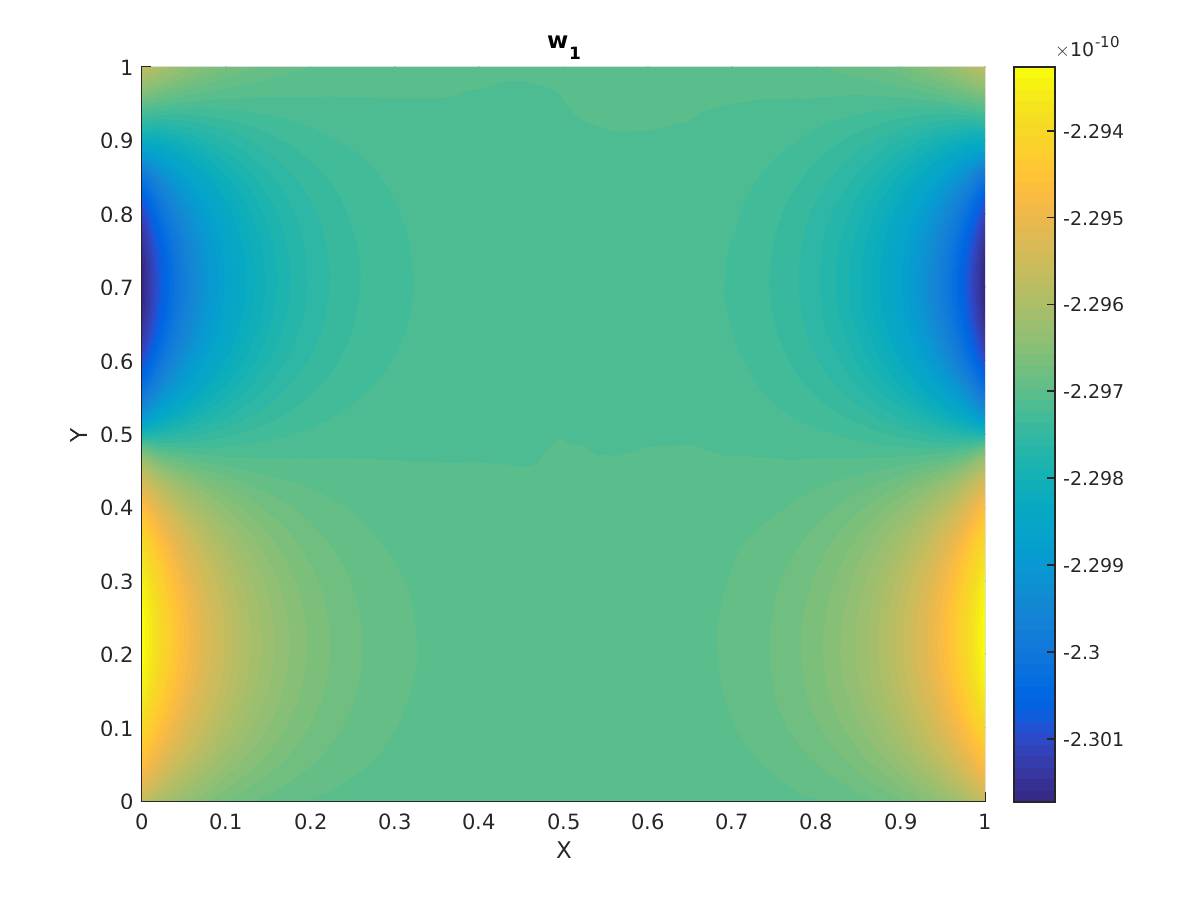
\includegraphics[height=.27\textheight]{SolutionPbHomogeneise/w1}
  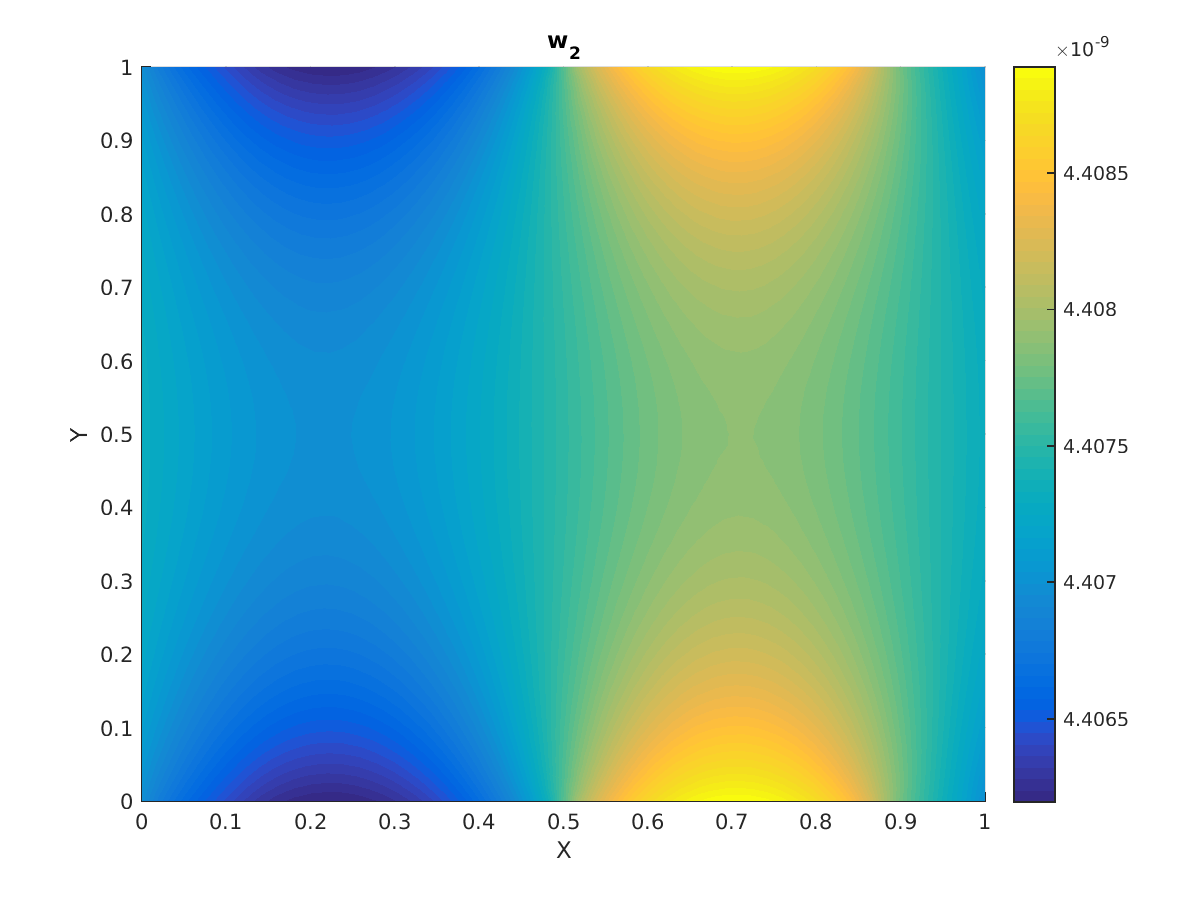
\includegraphics[height=.27\textheight]{SolutionPbHomogeneise/w2} 
  \caption{Solutions des problèmes de cellule pour le cas (ii), avec un maillage de $h=0.025$.}
  \label{fig:sol_pbcell}
\end{figure}


On retrouve bien les coefficients recherchés pour les cas (iii), (iv) et (v) comme prévu. Le reste du solveur étant le même que précédemment nous ne
referons pas les courbes de convergence en fonction du maillage pour cette partie là du code, on ne montrera pas non plus les résultats ainsi obtenus
puisqu'il s'agit d'un basique sinus. Cependant on pourra voir les différences entre solution homogène et solutions $\varepsilon$-dépendantes en
\autoref{fig:diffs} et les erreurs $L^2$ et $H^1$ associées en \autoref{fig;errhom}. On remarque que l'erreur $L^2$ décroît bien pour une gamme de
$\varepsilon$ mais commence à raugmenter à partir d'un certain $\varepsilon$ seuil. On pourrait attribuer cette erreur à la non résolution de
l'erreur, de plus que celle ci commence à apparaître qualitativement sur les graphes en même temps, même si on a vu en première partie que celle ci ne
semblait pas visible sur les courbes d'erreur. Pour vérifier cela on aimerait refaire les calculs avec un maillage plus fins, cependant mon ordinateur
n'est pas capable d'en gérer (manque de mémoire). On pourrait suggérer de travailler avec des maillage moins fins, cependant il ne semble pas y avoir
de différence sur les maillages ``proches'' et j'ai peur que de travailler avec des maillage beaucoup plus grossiers fassent apparaître d'autres types
d'erreur.

On observe aussi aisément que l'erreur $H^1$ ne converge pas, comme cela était annoncé par la théorie.



\begin{figure}
  \centering
  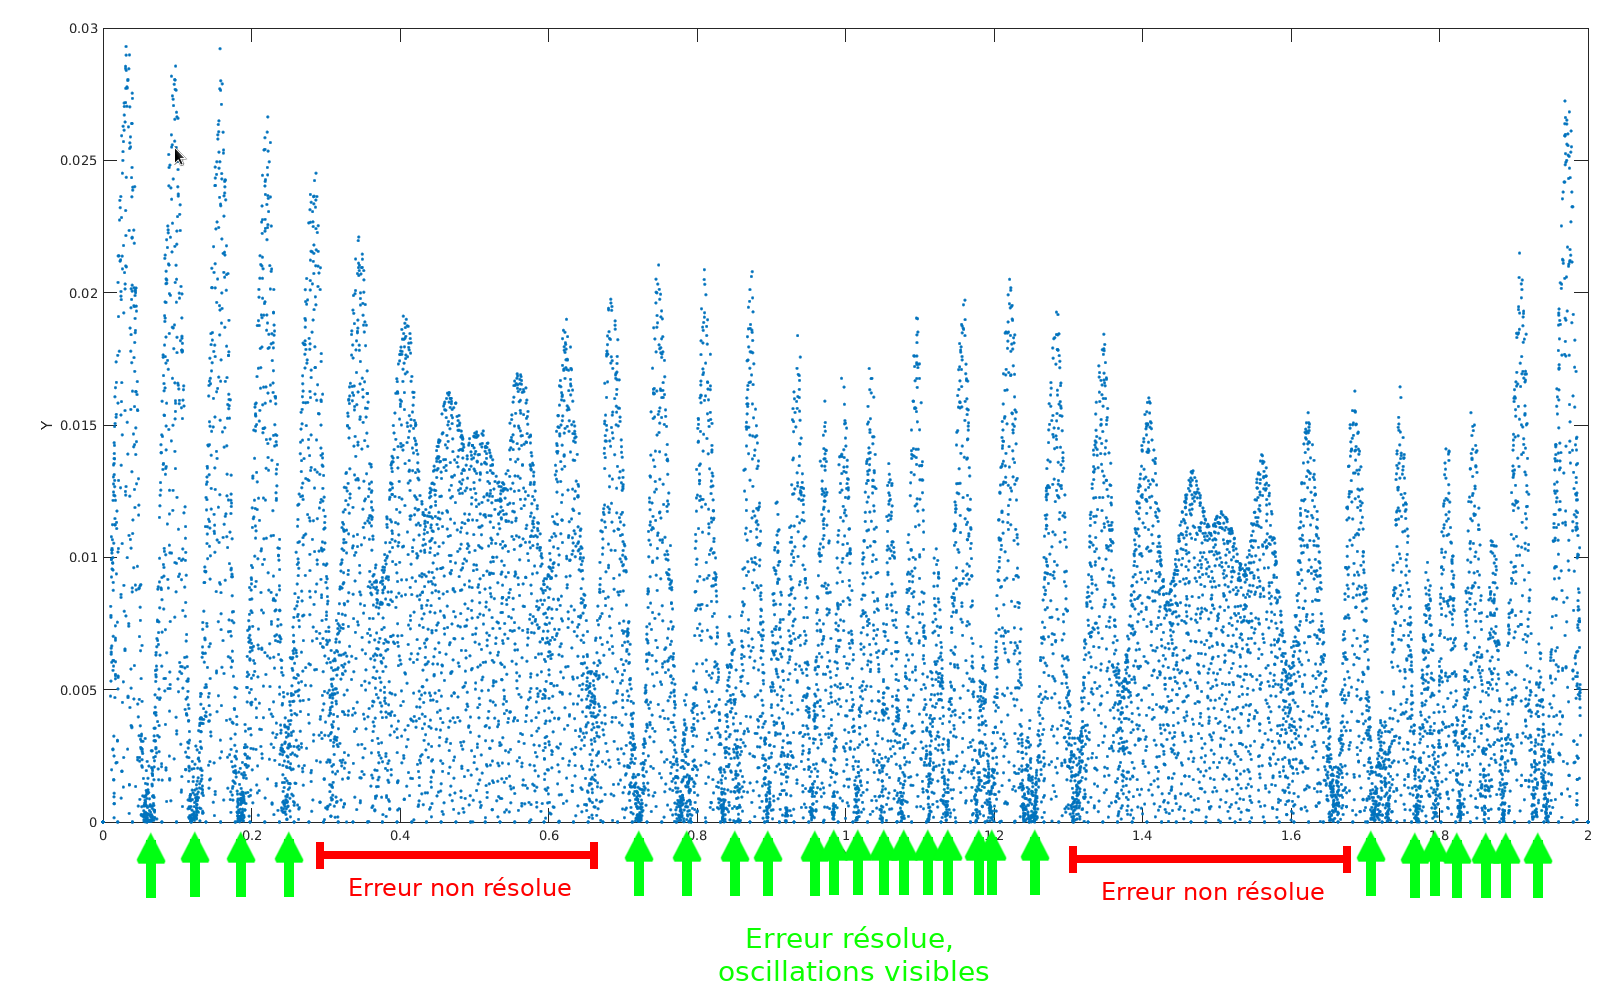
\includegraphics[width=.9\textwidth]{SolutionPbHomogeneise/non_res_osc}
  \caption{Profiles des erreurs en deux dimensions (panneaux supérieurs) et en fonction de l'abscisse (panneau inférieur).}
  \label{fig:diffs}
\end{figure}

\begin{figure}
  \centering
  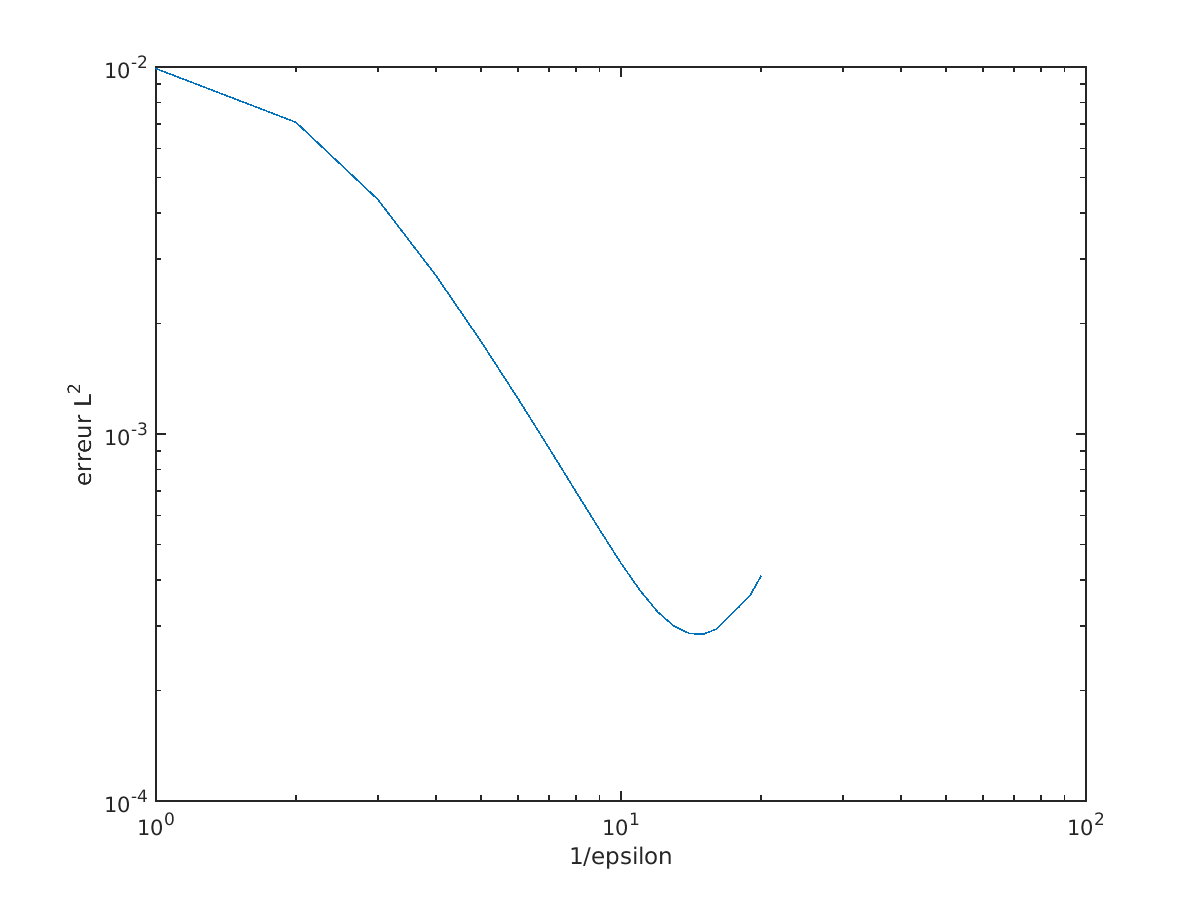
\includegraphics[height=.27\textheight]{SolutionPbHomogeneise/err_L2_eps}
  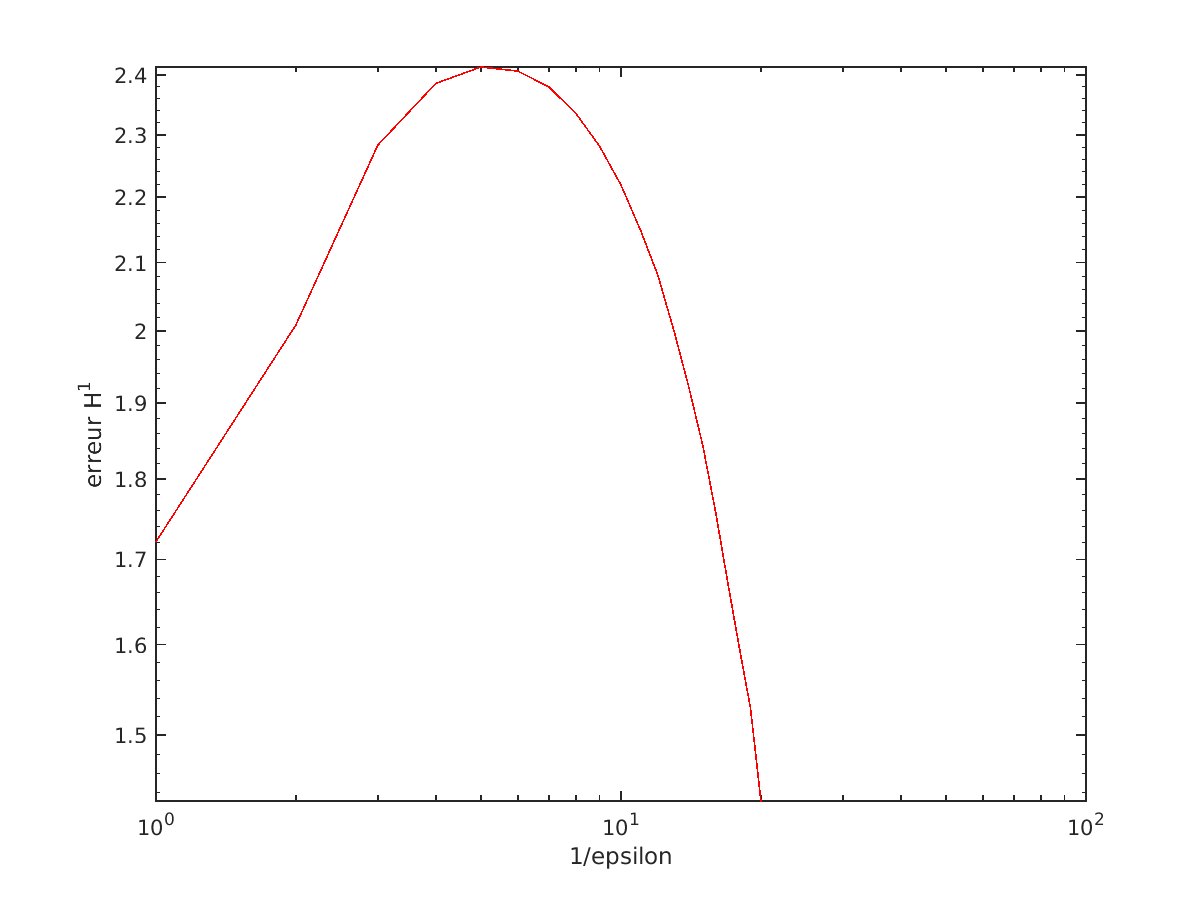
\includegraphics[height=.27\textheight]{SolutionPbHomogeneise/err_H1_eps} 
  \caption{Erreurs $L^2$ et $H^1$ par rapport à la solution homogénéisé en fonction de $\varepsilon$. On est ici dans le cas (îv), avec un maillage de
    $h=0.025$.}
  \label{fig:errhom}
\end{figure}

\end{document}

%%% Local Variables:
%%% mode: latex
%%% TeX-master: t
%%% End:
